\scanpage{72}
% archive sheet number: 71
% @ L1–9
Je voudrais revenir à la question de faire une surface avec les pos. \uline{stables}. Pour une telle $D$, $\Delta_D$ n'a comme arcs de transition que des arcs de \uline{spécialisation}. Comment raccorder $\Delta_D$ et $\Delta_{D'}$, quand $D,D'$ sont déduits l'un de l'autre par balayage au dessus d'un sommet ? Ici, il n'y

% @ L9–15, sketch between the two parts of the sentence
\figure{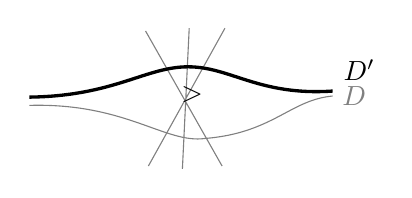
\begin{tikzpicture}[x=.72cm,y=.7cm]
\draw[gray] (-.6,-1.25)--(.75,1.25) (0,-1.3)--(.12,1.25) (.7,-1.25)--(-.65,1.2);
\draw[gray] (-2.7,-.15)..controls(-1,-.1)and(-.3,-.85)..(.4,-.75)..controls(1.6,-.65)and(1.9,-.05)..(2.65,.02) node[right]{$D$};
\draw[very thick] (-2.7,0)..controls(-1.2,.02)and(-.65,.55)..(.1,.55)..controls(.85,.55)and(1.35,.02)..(2.65,.11) node[above right]{$D'$};
\node at (.17,.05) {$>$};
\end{tikzpicture}}

% @ L9–20, text beside and below sketch
a pas d'ambiguïté possible sur les arcs le long desquels faire le vrillement, vu que l'interprétation de leur arc de spécialisation \unsure{n'en est plus une|n'est en plus une|et c'est plus utile} (il faudrait \unsure{du vis|du vice|du vif|être vicieux} pour l'utiliser pour vriller !). \margin{?} Ici, il est très tentant de remplacer encore $\Delta_D,\Delta_{D'}$ par $\Delta_D^*,\Delta_{D'}^*$ déduits en balayant le bord jusqu'au point $s$ ``critique'' qui nous intéresse, \deleted{avant} de vriller.

% @ L21–23 to R1–8
Résultat avec figures symétriques (à partir de la position \unsure{semi-stable|semi-stables|sous-stable} intermédiaire) on a à présent 8 possibilités

% @ R upper, two crossed drawings
\figure{\deleted{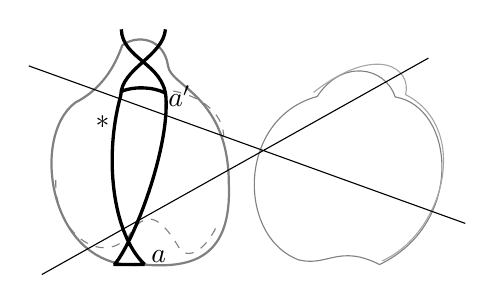
\begin{tikzpicture}[x=.66cm,y=.58cm]
\draw[gray,thick] (0,-2.2)..controls(-1.8,-2.4)and(-2.2,.6)..(-1.3,1.35)..controls(-.7,1.7)and(-.5,2.3)..(-.4,2.6)..controls(-.1,2.85)and(.4,2.75)..(.48,2.15)..controls(.52,1.7)and(1.65,1.5)..(1.65,-.45)..controls(1.7,-2)and(1,-2.3)..(0,-2.2);
\draw[gray,dashed] (-1.68,-.35)..controls(-1.72,-1.5)and(-.8,-2.25)..(-.28,-1.58)..controls(.05,-.95)and(.35,-1.15)..(.72,-1.89)..controls(1,-2.15)and(1.35,-1.6)..(1.45,-1.25) (.58,1.6)..controls(1.25,1.45)and(1.55,1)..(1.55,.6);
\draw[very thick] (-.42,2.95)..controls(-.4,2.3)and(.4,2.2)..(.44,1.45)..controls(.5,.35)and(-.15,-1.65)..(-.55,-2.2) (.43,2.95)..controls(.38,2.35)and(-.42,2.1)..(-.43,1.5)..controls(-.75,.2)and(-.61,-1.5)..(.03,-2.2) (-.42,1.59)..controls(-.2,1.7)and(.17,1.7)..(.42,1.56) (-.57,-2.2)--(.03,-2.2);
\node at (.7,1.48) {$a'$};\node at (.3,-2.02) {$a$};\node at (-.78,.92) {$*$};
\draw[gray] (3,-2.1)..controls(1.8,-1.6)and(1.8,1)..(3.35,1.48)..controls(3.82,2.3)and(4.65,2.15)..(4.85,1.47)..controls(6,1.25)and(6.2,-1.3)..(4.55,-2.2)..controls(3.77,-1.75)and(3.55,-2.25)..(3,-2.1);
\draw[gray!70] (3.28,1.57)..controls(4.5,2.65)and(5.18,2.1)..(5.05,1.52)..controls(6.3,.8)and(5.81,-1.5)..(4.6,-2.12);
\draw (-2.2,2.15)--(6.2,-1.3) (-1.95,-2.42)--(5.49,2.32);
\end{tikzpicture}}}

% @ R middle, redrawn pair of twists
\figure{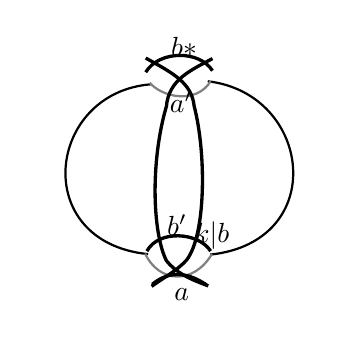
\begin{tikzpicture}[x=.75cm,y=.64cm]
\draw[thick] (-.48,1.53)..controls(-2.25,1.37)and(-2.55,-1.6)..(-.53,-1.84) (.48,1.59)..controls(2.25,1.35)and(2.55,-1.6)..(.52,-1.85);
\draw[gray,thick] (-.5,1.56)..controls(-.3,1.28)and(.28,1.12)..(.53,1.59) (-.58,-1.83)..controls(-.34,-2.42)and(.24,-2.45)..(.55,-1.84);
\draw[very thick] (-.57,2.05)..controls(-.12,1.76)and(.21,1.56)..(.25,1.1)..controls(.46,.15)and(.45,-1.47)..(.12,-1.96)..controls(-.04,-2.17)and(-.31,-2.34)..(-.47,-2.48) (.56,2.04)..controls(.18,1.8)and(-.18,1.62)..(-.22,1.09)..controls(-.49,.01)and(-.46,-1.4)..(-.22,-1.97)..controls(-.06,-2.2)and(.14,-2.32)..(.49,-2.47);
\draw[very thick] (-.57,1.77)..controls(-.34,2.21)and(.34,2.21)..(.56,1.8) (-.55,-1.78)..controls(-.35,-1.35)and(.32,-1.4)..(.53,-1.78) (-.46,-2.44)..controls(-.14,-2.13)and(.18,-2.23)..(.46,-2.45);
\node at (.08,2.28) {$b\deleted{*}$};\node at (.03,1.17) {$a'$};\node at (-.04,-1.26) {$b'$};\node at (.55,-1.47) {$\unsure{k|b}$};\node at (.04,-2.64) {$a$};
\end{tikzpicture}}

% @ R1–17 beside and below the redrawn figure
de vrillement, suivant les \deleted{qu'on} quatre choix d'\unsure{élémts|éléments} dans $\{a,a'\}\mathbin{\times}\{b,b'\}$, puis le choix d'orientation pour vriller $\alpha\in\{a,a'\}$ ou $\beta\in\{b,b'\}$. Mais déjà le choix d'un couple $(a,b')$ ou $(b,a')$ est exclu, à cause de la nécessaire symétrie à respecter. Donc il reste deux couples $(a,b)$, $(a',b')$, et pour chacun choix parmi les deux possibilités de vrillage -- transport parallèle, ou l'opposé. Mais modulo \deleted{application} transformation par antipodisme de part et d'autre (qui ne change pas la surface $X$ obtenue par vrillage \deleted{\unsure{suivant}} la disposition de la \deleted{\unsure{deux|droite|dedans}}) \unsure{DDS|reste|équivaut à} $(a,b)$.
